% Ensure that you compile using XeLaTeX !!! PDFTex has problems with some of the packages used
\documentclass[12pt]{article}
\setlength\parindent{0pt}

\usepackage{parskip}
\usepackage[margin=0.5in]{geometry}
\usepackage{fullpage}
\usepackage{moresize}
\usepackage{graphicx}
\usepackage{caption}
\usepackage{subcaption}
\usepackage{float}
\usepackage{xcolor}
\usepackage{soul}
\usepackage{fontspec}
\setmainfont{Doulos SIL}

\begin{document}

\begin{center}
\textbf{{\color{violet}{\HUGE 20201028 Wednesday\\}}}

\textbf{{\color{violet}{\HUGE ALL EXAMS (with notes)\\}}}

\end{center}
\newpage

\begin{center}
\textbf{{\color{blue}{\HUGE START OF EXAM\\}}}

\textbf{{\color{blue}{\HUGE Student ID: empty\\}}}

\textbf{{\color{blue}{\HUGE 10:00\\}}}

\end{center}
\newpage

\begin{center}
\textbf{{\color{blue}{\HUGE START OF EXAM\\}}}

\textbf{{\color{blue}{\HUGE Student ID: 36116\\}}}

\textbf{{\color{blue}{\HUGE 10:10\\}}}

\end{center}
\newpage

{\large Question 1}\\

Topic: Articulatory Phonetics\\
Source: Week 3 Discussion\\

Assuming a Standard North American English inventory, does this vowel need to have tenseness specified if you're giving a prose description? Why or why not?\\

{[ɑ]}


~\\
INSTRUCTOR NOTES: no


\vfill
Excellent (3) ~~~ Good (2.2) ~~~ Fair (1.7) ~~~ Poor (0)
\newpage

{\large Question 2}\\

Topic: Phonological Features\\
Source: Week 4 Discussion\\

Explain why phonological features are used instead of phonetic characteristics in analyzing datasets.\\


~\\
INSTRUCTOR NOTES: Phonological features help to capture phonological patterns, i.e., they group sounds together based on whether they do things like triggering a change or undergoing a change. Phonological features are sometimes language-specific. Phonetic characteristics are simply descriptions of the physical properties of the sounds; they are language-universal and independent of the patterns (though it turns out that many phonological patterns are based on phonetic characteristic groupings).


\vfill
Excellent (3) ~~~ Good (2.2) ~~~ Fair (1.7) ~~~ Poor (0)
\newpage

\begin{center}
\textbf{{\color{red}{\HUGE END OF EXAM}}}\\

\end{center}
\newpage

\begin{center}
\textbf{{\color{blue}{\HUGE START OF EXAM\\}}}

\textbf{{\color{blue}{\HUGE Student ID: 83841\\}}}

\textbf{{\color{blue}{\HUGE 10:20\\}}}

\end{center}
\newpage

{\large Question 1}\\

Topic: Other (pre-midterm)\\
Source: Week 4 Handout, Part II, Question 2(iii)\\

Explain how you would figure out the meaning of this Swahili word. (To be clear: you do NOT need to give me the meaning itself -- just explain the process of figuring it out.)\\

{[watanipiɡa]}

\begin{figure}[H]
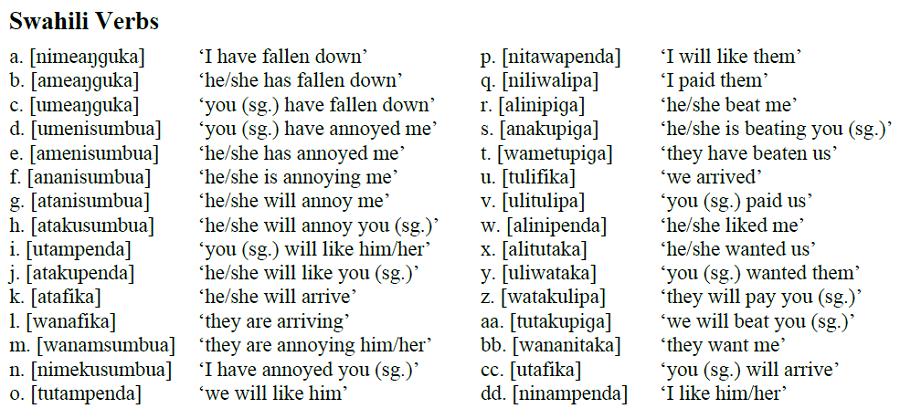
\includegraphics{../images/swahiliverbs.png}
\end{figure}

~\\
INSTRUCTOR NOTES: (they will beat me)


\vfill
Excellent (3) ~~~ Good (2.2) ~~~ Fair (1.7) ~~~ Poor (0)
\newpage

{\large Question 2}\\

Topic: Phonological Features\\
Source: Quiz 3, Question 12\\

Explain how you figure out which feature is involved in the process of umlaut shown below.\\

\begin{figure}[H]
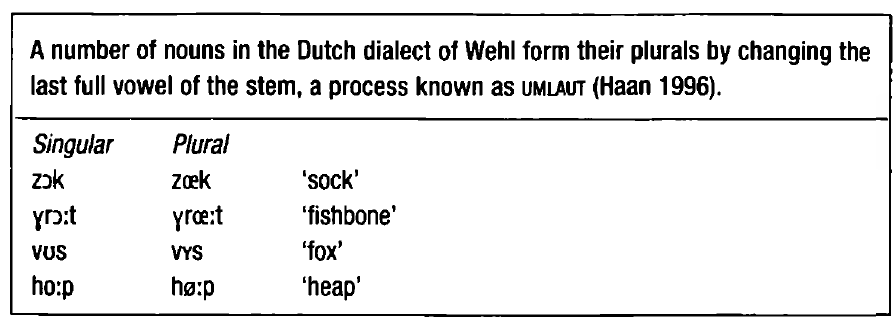
\includegraphics{../images/dutch.png}
\end{figure}

~\\
INSTRUCTOR NOTES: we look to see which vowels are affected, and compare them to see which feature is DIFFERENT (not e.g. what features they share); so since the vowels in the singular and plural are identical except that the singular forms are back and the plural are front, it's the feature [back] that is relevant / changing / involved (not e.g. the feature [round] just because all of the vowels are round)


\vfill
Excellent (3) ~~~ Good (2.2) ~~~ Fair (1.7) ~~~ Poor (0)
\newpage

\begin{center}
\textbf{{\color{red}{\HUGE END OF EXAM}}}\\

\end{center}
\newpage

\begin{center}
\textbf{{\color{blue}{\HUGE START OF EXAM\\}}}

\textbf{{\color{blue}{\HUGE Student ID: 74752\\}}}

\textbf{{\color{blue}{\HUGE 10:30\\}}}

\end{center}
\newpage

{\large Question 1}\\

Topic: Transcription\\
Source: Week 2 Handout, Part II\\

Is this a reasonable transcription of this word? Explain why.\\

<wimp>: {[wimp]}


~\\
INSTRUCTOR NOTES: no, [ɪ]


\vfill
Excellent (3) ~~~ Good (2.2) ~~~ Fair (1.7) ~~~ Poor (0)
\newpage

{\large Question 2}\\

Topic: Articulatory Phonetics\\
Source: Quiz 2, Question 6\\

In the pronunciation of this word, which sounds are obstruents and which are sonorants? Explain your answer.\\

<sonorant>


~\\
INSTRUCTOR NOTES: [sɔnoɹənt] -- sonorants: [ɔnoɹən] and obstruents: [st]


\vfill
Excellent (3) ~~~ Good (2.2) ~~~ Fair (1.7) ~~~ Poor (0)
\newpage

\begin{center}
\textbf{{\color{red}{\HUGE END OF EXAM}}}\\

\end{center}
\newpage

\begin{center}
\textbf{{\color{blue}{\HUGE START OF EXAM\\}}}

\textbf{{\color{blue}{\HUGE Student ID: 17335\\}}}

\textbf{{\color{blue}{\HUGE 10:40\\}}}

\end{center}
\newpage

{\large Question 1}\\

Topic: Skewed Distributions\\
Source: Week 5 Handout, Question 5\\

Explain why looking for patterns with consonants and vowels is a more reasonable approach to pattern finding in this dataset than looking for patterns with respect to all of the individual sounds in Ukrainian.\\

\begin{figure}[H]
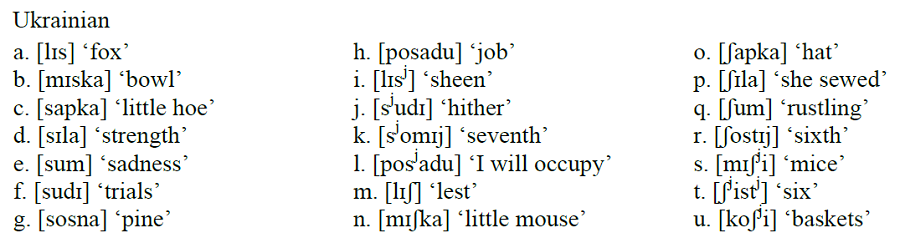
\includegraphics{../images/ukrainian.png}
\end{figure}

~\\
INSTRUCTOR NOTES: Collapsing sounds into "consonants" and "vowels" allows us to have 'sufficient data' in a way that thinking about all the individual combinations of sounds would not.


\vfill
Excellent (3) ~~~ Good (2.2) ~~~ Fair (1.7) ~~~ Poor (0)
\newpage

{\large Question 2}\\

Topic: Other (pre-midterm)\\
Source: Week 4 Handout, Part II, Question 3\\

Explain how you would figure out what the Luiseño form is for the morpheme whose meaning is given below. (To be clear: you do NOT need to give me the form itself -- just explain the process of figuring it out.)\\

‘drink’

\begin{figure}[H]
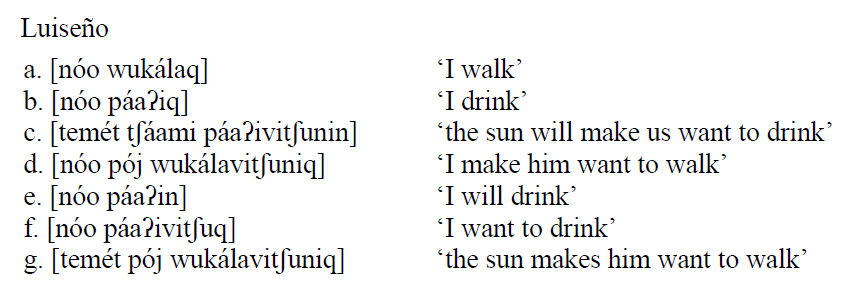
\includegraphics{../images/luiseno.png}
\end{figure}

~\\
INSTRUCTOR NOTES: ([páaʔi])


\vfill
Excellent (3) ~~~ Good (2.2) ~~~ Fair (1.7) ~~~ Poor (0)
\newpage

\begin{center}
\textbf{{\color{red}{\HUGE END OF EXAM}}}\\

\end{center}
\newpage

\begin{center}
\textbf{{\color{blue}{\HUGE START OF EXAM\\}}}

\textbf{{\color{blue}{\HUGE Student ID: empty\\}}}

\textbf{{\color{blue}{\HUGE 10:50\\}}}

\end{center}
\newpage

\begin{center}
\textbf{{\color{blue}{\HUGE START OF EXAM\\}}}

\textbf{{\color{blue}{\HUGE Student ID: 33446\\}}}

\textbf{{\color{blue}{\HUGE 4:00\\}}}

\end{center}
\newpage

{\large Question 1}\\

Topic: Articulatory Phonetics\\
Source: Week 3 Handout, Question 3\\

Explain why the additional vowel below either does or does not belong in the phonetic natural class defined by the original set of SNAE vowels.\\

Original set: {[æ]}, {[ɑ]}

Addition: {[ɑʊ]}


~\\
INSTRUCTOR NOTES: should recognize that there's more than one vowel sound, which makes it somewhat difficult to categorize; best answers will say that the diphthong is crucially a diphthong and so can't also go in this class


\vfill
Excellent (3) ~~~ Good (2.2) ~~~ Fair (1.7) ~~~ Poor (0)
\newpage

{\large Question 2}\\

Topic: Skewed Distributions\\
Source: Quiz 4, Question 1\\

L$_X$ (Language X) has three vowels, [i], [a], and [u]. It has bi-syllabic roots like Kikuyu. It does not allow non-identical high vowels to co-occur. Of the following nine logically possible vocalic sequences, which ones should be unattested in L$_X$? Explain why.\\

\begin{itemize} \item {[i...i]} \item {[i...a]} \item {[i...u]} \item {[a...i]} \item {[a...a]} \item {[a...u]} \item {[u...i]} \item {[u...a]} \item {[u...u]} \end{itemize}


~\\
INSTRUCTOR NOTES: [i...u], [u...i]


\vfill
Excellent (3) ~~~ Good (2.2) ~~~ Fair (1.7) ~~~ Poor (0)
\newpage

\begin{center}
\textbf{{\color{red}{\HUGE END OF EXAM}}}\\

\end{center}
\newpage

\begin{center}
\textbf{{\color{blue}{\HUGE START OF EXAM\\}}}

\textbf{{\color{blue}{\HUGE Student ID: 27762\\}}}

\textbf{{\color{blue}{\HUGE 4:10\\}}}

\end{center}
\newpage

{\large Question 1}\\

Topic: Articulatory Phonetics\\
Source: Week 3 Discussion\\

Assuming a Standard North American English inventory, does this vowel need to have tenseness specified if you're giving a prose description? Why or why not?\\

{[i]}


~\\
INSTRUCTOR NOTES: yes


\vfill
Excellent (3) ~~~ Good (2.2) ~~~ Fair (1.7) ~~~ Poor (0)
\newpage

{\large Question 2}\\

Topic: Phonological Features\\
Source: Quiz 3, Question 12\\

Explain how you figure out which feature is involved in the process of umlaut shown below.\\

\begin{figure}[H]
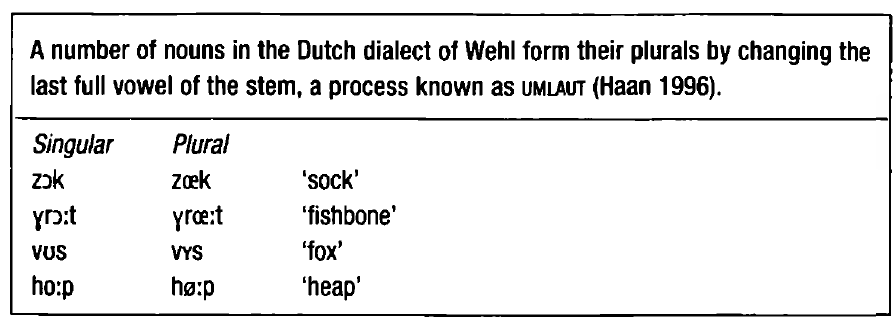
\includegraphics{../images/dutch.png}
\end{figure}

~\\
INSTRUCTOR NOTES: we look to see which vowels are affected, and compare them to see which feature is DIFFERENT (not e.g. what features they share); so since the vowels in the singular and plural are identical except that the singular forms are back and the plural are front, it's the feature [back] that is relevant / changing / involved (not e.g. the feature [round] just because all of the vowels are round)


\vfill
Excellent (3) ~~~ Good (2.2) ~~~ Fair (1.7) ~~~ Poor (0)
\newpage

\begin{center}
\textbf{{\color{red}{\HUGE END OF EXAM}}}\\

\end{center}
\newpage

\begin{center}
\textbf{{\color{blue}{\HUGE START OF EXAM\\}}}

\textbf{{\color{blue}{\HUGE Student ID: 52421\\}}}

\textbf{{\color{blue}{\HUGE 4:20\\}}}

\end{center}
\newpage

{\large Question 1}\\

Topic: Skewed Distributions\\
Source: Week 5 Handout, Question 5\\

Explain why looking for patterns with consonants and vowels is a more reasonable approach to pattern finding in this dataset than looking for patterns with respect to all of the individual sounds in Ukrainian.\\

\begin{figure}[H]
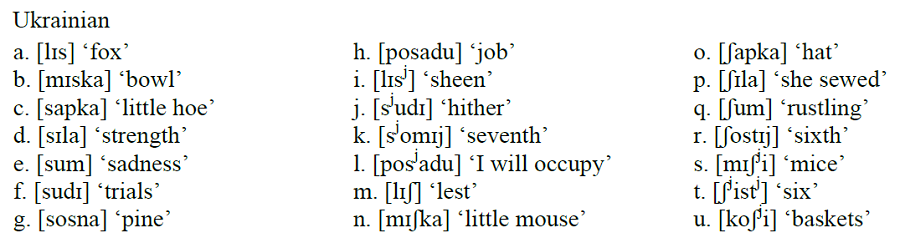
\includegraphics{../images/ukrainian.png}
\end{figure}

~\\
INSTRUCTOR NOTES: Collapsing sounds into "consonants" and "vowels" allows us to have 'sufficient data' in a way that thinking about all the individual combinations of sounds would not.


\vfill
Excellent (3) ~~~ Good (2.2) ~~~ Fair (1.7) ~~~ Poor (0)
\newpage

{\large Question 2}\\

Topic: Transcription\\
Source: Week 2 Handout, Part II, Question 11\\

How would this word be transcribed?\\ (Kathleen will then ask a follow-up question about your transcription.)\\

<toy>


~\\
INSTRUCTOR NOTES: [tɔɪ]


\vfill
Excellent (3) ~~~ Good (2.2) ~~~ Fair (1.7) ~~~ Poor (0)
\newpage

\begin{center}
\textbf{{\color{red}{\HUGE END OF EXAM}}}\\

\end{center}
\newpage

\begin{center}
\textbf{{\color{blue}{\HUGE START OF EXAM\\}}}

\textbf{{\color{blue}{\HUGE Student ID: 56567\\}}}

\textbf{{\color{blue}{\HUGE 4:30\\}}}

\end{center}
\newpage

{\large Question 1}\\

Topic: Skewed Distributions\\
Source: Quiz 4, Question 2\\

L$_X$ (Language X) has three vowels, [i], [a], and [u]. L$_X$ has tri-syllabic roots. If L$_X$ does not allow non-identical high vowels to co-occur, which one of the following tri-syllabic vocalic sequences do you predict to be unattested in L$_X$? Explain why.\\

\begin{itemize} \item {[u...i...a]} \item {[a...i...a]} \item {[u...u...a]} \item {[a...i...i]} \end{itemize}


~\\
INSTRUCTOR NOTES: [u...i...a]


\vfill
Excellent (3) ~~~ Good (2.2) ~~~ Fair (1.7) ~~~ Poor (0)
\newpage

{\large Question 2}\\

Topic: Other (pre-midterm)\\
Source: Week 5 \& 6 Handouts\\

Explain how you could analyze this dataset in terms of sequential patterns vs. paradigmatic patterns.\\

\begin{figure}[H]
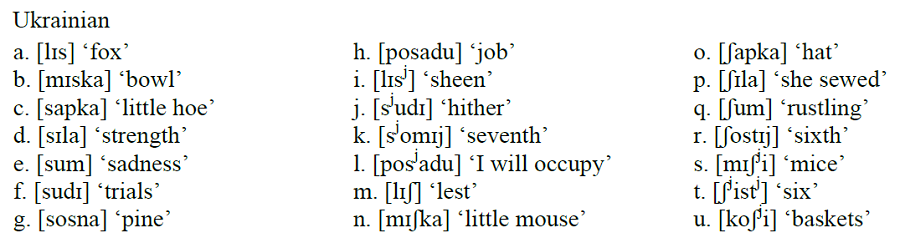
\includegraphics{../images/ukrainian.png}
\end{figure}

~\\
INSTRUCTOR NOTES: 


\vfill
Excellent (3) ~~~ Good (2.2) ~~~ Fair (1.7) ~~~ Poor (0)
\newpage

\begin{center}
\textbf{{\color{red}{\HUGE END OF EXAM}}}\\

\end{center}
\newpage

\begin{center}
\textbf{{\color{blue}{\HUGE START OF EXAM\\}}}

\textbf{{\color{blue}{\HUGE Student ID: 36273\\}}}

\textbf{{\color{blue}{\HUGE 4:40\\}}}

\end{center}
\newpage

{\large Question 1}\\

Topic: Phonological Features\\
Source: Quiz 3, Question 12\\

Explain how you figure out which feature is involved in the process of umlaut shown below.\\

\begin{figure}[H]
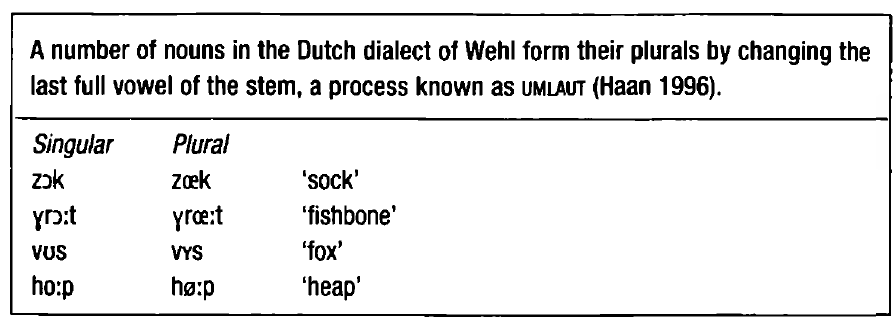
\includegraphics{../images/dutch.png}
\end{figure}

~\\
INSTRUCTOR NOTES: we look to see which vowels are affected, and compare them to see which feature is DIFFERENT (not e.g. what features they share); so since the vowels in the singular and plural are identical except that the singular forms are back and the plural are front, it's the feature [back] that is relevant / changing / involved (not e.g. the feature [round] just because all of the vowels are round)


\vfill
Excellent (3) ~~~ Good (2.2) ~~~ Fair (1.7) ~~~ Poor (0)
\newpage

{\large Question 2}\\

Topic: Skewed Distributions\\
Source: Quiz 4, Question 1\\

L$_X$ (Language X) has three vowels, [i], [a], and [u]. It has bi-syllabic roots like Kikuyu. It does not allow non-identical high vowels to co-occur. Of the following nine logically possible vocalic sequences, which ones should be unattested in L$_X$? Explain why.\\

\begin{itemize} \item {[i...i]} \item {[i...a]} \item {[i...u]} \item {[a...i]} \item {[a...a]} \item {[a...u]} \item {[u...i]} \item {[u...a]} \item {[u...u]} \end{itemize}


~\\
INSTRUCTOR NOTES: [i...u], [u...i]


\vfill
Excellent (3) ~~~ Good (2.2) ~~~ Fair (1.7) ~~~ Poor (0)
\newpage

\begin{center}
\textbf{{\color{red}{\HUGE END OF EXAM}}}\\

\end{center}
\newpage

\begin{center}
\textbf{{\color{blue}{\HUGE START OF EXAM\\}}}

\textbf{{\color{blue}{\HUGE Student ID: 19711\\}}}

\textbf{{\color{blue}{\HUGE 4:50\\}}}

\end{center}
\newpage

{\large Question 1}\\

Topic: Transcription\\
Source: Week 2 Handout, Part II, Question 11\\

How would this word be transcribed?\\ (Kathleen will then ask a follow-up question about your transcription.)\\

<juice>


~\\
INSTRUCTOR NOTES: [dʒus]


\vfill
Excellent (3) ~~~ Good (2.2) ~~~ Fair (1.7) ~~~ Poor (0)
\newpage

{\large Question 2}\\

Topic: Skewed Distributions\\
Source: Week 5 Handout, Question 7\\

Explain how you would go about looking for co-occurrence restrictions in bi-syllabic signs in ASL. (Refer to the data that follows.)\\

\begin{figure}[H]
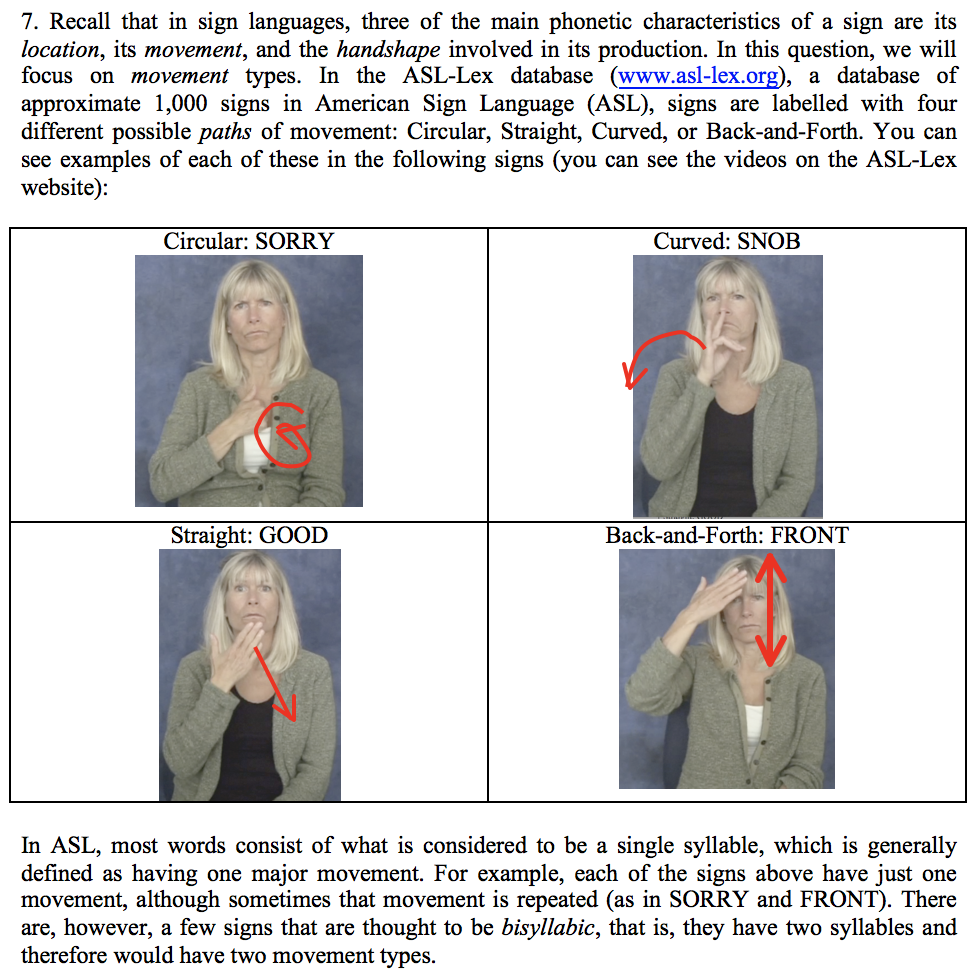
\includegraphics{../images/ASL_movement.png}
\end{figure}

~\\
INSTRUCTOR NOTES: You would start by coming up with all the possible combinations expected (i.e., 4x4 = 16). Then you'd compare that to some database of signs in ASL and see which combinations are actually attested or unattested.


\vfill
Excellent (3) ~~~ Good (2.2) ~~~ Fair (1.7) ~~~ Poor (0)
\newpage

\begin{center}
\textbf{{\color{red}{\HUGE END OF EXAM}}}\\

\end{center}
\newpage

\end{document}

